% !TEX root = ../thesis-main.tex

\acresetall

\chapter{Generative Recommendations with Diffusion}
%\chapter{Counterfactual Explanations for Graphs}
\label{chapter:research-recfusion}

\footnote[]{This chapter is under submission at International Conference on Learning Representations (ICLR) under the title ``RecFusion: A Binomial Diffusion Process for 1D Data for Recommendation'' \citep{lucic2021cfgnnexplainer}.}
\acresetall

%\todo{Add intro paragraph that connects this chapter to its RQ from chapter 1: How can we extend our explanation method for tree-based models to graph-based models? first extend problem formalization to graphs, then apply the same gradient-based optimization technique as in FOCUS}

\medskip
\noindent
\textbf{\ref{rq:recfusion}:} \acl{rq:recfusion}
\medskip

\noindent

\subimport{recfusion-arxiv/sections}{01_introduction}
\subimport{recfusion-arxiv/sections}{02_method}
\subimport{recfusion-arxiv/sections}{03_experimental_setup}
\subimport{recfusion-arxiv/sections}{04_results}
\subimport{recfusion-arxiv/sections}{05_related_work}
\subimport{recfusion-arxiv/sections}{06_discussion}

\begin{appendices}
\chapter{Appendix of Generative Recommendations with Diffusion}
\subimport{recfusion-arxiv}{appendix}
\end{appendices}

%\input{04-research-recfusion/recfusion-arxiv/sections/01_introduction}

%\include{04-research-recfusion/recfusion-arxiv/sections/01_introduction}

%%!TEX root = ../main.tex


\section{Introduction}
\label{section:fact-introduction}

For several decades, \OurUniversity{} has offered a research-oriented Master of Science (MSc) program in AI. 
The main focus of the program is on the technical machine learning (ML) aspects of the major sub-fields of AI, such as computer vision, information retrieval, natural language processing, and reinforcement learning.
One of the most recent additions to the MSc AI curriculum is a mandatory course called \emph{\ac{FACT-AI}}. 
This course was first taught during the 2019--2020 academic year and focuses on teaching FACT-AI topics through the lens of reproducibility. 
The main project involves students working in groups to re-implement existing FACT-AI algorithms from papers in top AI venues. 
There are approximately 150 students enrolled in the course each year. 

The motivation for the course came from the MSc AI students themselves, who often play an important role in shaping the curriculum in order to meet the evolving requirements of researchers in both academia and industry. 
As the influence of AI on decision making is becoming increasingly prevalent in day-to-day life, there is a growing consensus that stakeholders who take part in the design or implementation of AI algorithms should reflect on the ethical ramifications of their work, including developers and researchers \citep{campbell2021_responsible}. 
This is especially true in situations where data-driven AI systems affect some demographic sub-groups differently than others \citep{propublica, o2017ivory}.
As a result, our students have shown an increased interest in the ethical issues surrounding AI systems and requested that the university put together a new course focusing on responsible AI.

Since our MSc AI program is characterized by a strong emphasis on understanding, developing, and building AI algorithms, we believe that a new course on responsible AI in this program should also have a hands-on approach.
The course is designed to address technical aspects of key areas in responsible AI:
\begin{enumerate*}[label=(\roman*)]
\item fairness, 
\item accountability, 
\item confidentiality, and 
\item transparency,  
\end{enumerate*}
which we operationalize through a reproducibility project. 
We believe a strong emphasis on reproducibility is important from both an educational point of view and from the point of view of the AI community, since the (lack of) reproducible results has become a major point of critique in AI \citep{hutson2018artificial}. 
Moreover, the starting point of almost any junior AI researcher (and most AI research projects in general) is re-implementing existing methods as baselines. 
The FACT-AI course is situated at a point in the program where students have learned the basics of ML and are ready to start experimenting with, and building on top of, state-of-the-art algorithms. 
Given that our MSc AI program is fairly research-oriented, it is important for students to experience the process of reproducing work done by others (and how difficult this is) at an early stage in their careers. 
We also believe reproducibility is a fundamental component of FACT-AI: the cornerstone of fair, accountable, confidential and transparent AI systems is having correct and reproducible results. 
Without reproducibility, it is unclear how to judge if a decision-making algorithm adheres to any of the FACT principles. 

In the 2019--2020 academic year, we operationalized our learning ambitions regarding reproducibility by publishing a public repository with selected code implementations and corresponding reports from the group projects.
In the 2020--2021 academic year, we took the projects one step further and encouraged students to submit to the ML Reproducibility Challenge,\footnote{\url{https://paperswithcode.com/rc2020}} a competition that solicits reproducibility reports for papers published in conferences such as NeurIPS, ICML, ICLR, ACL, EMNLP, CVPR and ECCV. 
Although the challenge broadly focuses on all papers submitted to these conferences, we focus exclusively on papers covering FACT-AI topics in our course. 
Submitting to the challenge gives students a chance to experience the whole AI research pipeline, from running experiments, to writing rebuttals, to receiving the official notifications. 
Of the 23 papers that were accepted to the ML Reproducibility Challenge in 2021, 9 came from groups in the FACT-AI course. 

In this chapter, we describe the FACT-AI course at \OurUniversity{}: a one month, full-time course based on examining ethical issues in AI using reproducibility as a pedagogical tool. 
Students work in groups to re-implement (and possibly extend) existing algorithms from top AI venues on \ac{FACT-AI} topics. 
The course also includes lectures that cover the high-level principles of FACT-AI topics, as well as paper discussion sessions where students read and digest prominent FACT-AI papers. 
In this chapter, we outline the setup for the \ac{FACT-AI} course and the experiences we had while running the course during the 2019--2020 and 2020--2021 academic years at \OurUniversity{}. 

The remainder of this chapter is structured as follows. 
In Section~\ref{section:fact-related-work}, we discuss related work, specifically other courses about responsible AI. 
In Section~\ref{section:reproducibility}, we detail ongoing reproducibility efforts in the AI community. 
In Section~\ref{section:learning-objectives}, we explain the learning objectives for our course, and explain how we realized those objectives in Section~\ref{section:coursesetup}. 
We reflect on the feedback we received about the course in Section~\ref{section:feedback}, as well as what worked (Section~\ref{section:whatworked}) and what did not (Section~\ref{section:whatdidnt}), before concluding in Section~\ref{section:fact-conclusion}. 

%%!TEX root = ../main.tex

\section{Related Work}
\label{section:focus-related-work}
Based on the taxonomy described in Chapter~\ref{chapter:introduction}, our setting in this chapter is a \emph{local explanation} problem for \emph{tree ensembles}. 
We use \emph{sensitivity analysis}, specifically counterfactual perturbations, on \emph{tabular} data to generate our explanations. 
Our work is related to counterfactual explanations in general (Section~\ref{section:focus-cf}), algorithmic recourse (Section~\ref{section:focus-recourse}), adversarial examples (Section~\ref{section:focus-adversarial}), and differentiable tree-based models (Section~\ref{section:focus-diff-trees}).

\subsection{Counterfactual Explanations}
\label{section:focus-cf}
Counterfactual examples have been used in a variety of ML areas, such as reinforcement learning \citep{madumal_explainable_2019}, deep learning \citep{alaa_deep_2017}, and XAI. 
Previous XAI methods for generating counterfactual examples are either model-agnostic \citep{poyiadzi_face_2020, karimi_model-agnostic_2019, laugel_inverse_2017, van_looveren_interpretable_2020,  mothilal_explaining_2020} or model-specific \citep{wachter_counterfactual_2017, grath_interpretable_2018, tolomei_interpretable_2017, kanamori_dace_2020, russell_efficient_2019, dhurandhar_explanations_2018}. 
Model-agnostic approaches treat the original model as a ``black-box'' and only assume query access to the model, whereas model-specific approaches typically do not make this assumption and can therefore make use of its inner workings (see Chapter~\ref{chapter:introduction}). 

Our work is a model-specific approach for generating counterfactual examples through optimization. 
Previous model-specific work for generating counterfactual examples through optimization has solely been conducted on differentiable models \citep{wachter_counterfactual_2017, grath_interpretable_2018, dhurandhar_explanations_2018}. 

\subsection{Algorithmic Recourse}
\label{section:focus-recourse}
Algorithmic recourse is a line of research that is closely related to counterfactual explanations, except that methods for algorithmic recourse include the additional restriction that the resulting explanation must be \emph{actionable} \citep{ustun_actionable_2019, joshi_towards_2019, karimi_recourse_2020, karimi_imperfect_causal_2020}. 
This is done by selecting a subset of the features to which perturbations can be applied in order to avoid explanations that suggest impossible or unrealistic changes to the feature values (i.e., change \textit{age} from \numprint{50} $\to$ \numprint{25}). 
Although this work has produced impressive theoretical results, it is unclear how realistic they are in practice, especially for complex ML models such as tree ensembles. 
Existing algorithmic recourse methods cannot solve our task because they 
\begin{enumerate*}[label=(\roman*)]
	\item are either restricted to solely linear \citep{ustun_actionable_2019} or  differentiable \citep{joshi_towards_2019} models, or
	\item  require access to causal information \citep{karimi_recourse_2020, karimi_imperfect_causal_2020}, which is rarely available in real world settings. 
\end{enumerate*}

\subsection{Adversarial Examples}
\label{section:focus-adversarial}
Adversarial examples are a type of counterfactual example with the additional constraint that the minimal perturbation results in an alternative prediction that is \emph{incorrect}. 
There are a variety of methods for generating adversarial examples \citep{goodfellow_explaining_2015,szegedy_intriguing_2014,su_one_2019,brown_adversarial_2018}; a more complete overview can be found in the work of \cite{biggio_wild_2018}. 
The main difference between adversarial examples and counterfactual examples is in the intent: adversarial examples are meant to \emph{fool} the model, whereas counterfactual examples are meant to \emph{explain} the model.


\subsection{Differentiable Tree-based Models}
\label{section:focus-diff-trees}
Part of our contribution involves constructing differentiable versions of tree ensembles by replacing each splitting threshold with a sigmoid function. 
This can be seen as using a (small) neural network to obtain a smooth approximation of each tree. 
Neural decision trees \citep{balestriero_neural_2017, yang_deep_2018} are also differentiable versions of trees, which use a full neural network instead of a simple sigmoid. 
However, these do not optimize for approximating an already trained model. Therefore, unlike our method, they are not an obvious choice for finding counterfactual examples for an existing model. 
Soft decision trees~\citep{hinton_distilling_2014} are another example of differentiable trees, which instead approximate a neural network with a decision tree. 
This can be seen as the inverse of our task. 


%%!TEX root = ../main.tex

\section{Background}
\label{section:background}
In this section, we provide background information on GNNs (Section~\ref{section:gnns-general}) and matrix sparsification (Section~\ref{section:matrix-sparsification}), both of which are necessary for understanding CF-GNNExplainer. 

\subsection{Graph Neural Networks}
\label{section:gnns-general}
Graphs are structures that represent a set of entities (nodes) and their relations (edges). 
GNNs operate on graphs to produce representations that can be used in downstream tasks such as graph or node classification. The latter is the focus of this work.
We refer to the survey papers by \citet{battaglia_relational_2018} and \citet{chami2021machine} for an overview of existing GNN methods. 

Let $f(A, X; W) \rightarrow y$ be any GNN, where $y$ is the set of possible predicted classes, $A$ is an $n \times n$ adjacency matrix, $X$ is an $n \times p$ feature matrix, and $W$ is the learned weight matrix of $f$. 
In other words, $A$ and $X$ are the inputs of $f$, and $f$ is parameterized by $W$. 

A node's representation is learned by iteratively updating the node's features based on its neighbors' features.   
The number of layers in $f$ determines which neighbors are included: if there are $\ell$ layers, then the node's final representation only includes neighbors that are at most $\ell$ hops away from that node in the graph $\graph$. 
The rest of the nodes in $\graph$ are not relevant for the computation of the node's final representation.  
We define the \emph{\cgraph{}} of a node $v$ as the set of the nodes and edges relevant for the computation of $f(v)$ (i.e., those in the $\ell$-hop neighborhood of $f$), represented as a tuple: $\compgraph = (\compadj, \compnode)$, where $\compadj$ is the subgraph adjacency matrix and $X_v$ is the node feature matrix for nodes that are at most $\ell$ hops away from $v$. We then define a node $v$ as a tuple of the form $v = (\compadj, x)$, where $x$ is the feature vector for $v$. 

\subsection{Matrix Sparsification}
\label{section:matrix-sparsification}
CF-GNNExplainer uses matrix sparsification to generate counterfactual examples, inspired by~\citet{srinivas_training_2016}, who propose a method for training sparse neural networks. 
Given a weight matrix $W$, a binary sparsification matrix is learned which is multiplied element-wise with $W$ such that some of the entries in $W$ are zeroed out. 
In the work by \citet{srinivas_training_2016}, the objective is to remove entries in the weight matrix in order to reduce the number of parameters in the model. 
In our case, we want to \emph{zero out entries in the adjacency matrix} (i.e., remove edges) in order to generate counterfactual explanations for GNNs. 
That is, we want to remove the important edges -- those that are crucial for the prediction. 
%%!TEX root = ../main.tex

\section{Problem Formulation}
\label{section:problem-formulation}
In general, a counterfactual example $\bar{x}$ for an instance $x$ according to a trained classifier $f$ is found by perturbing the features of $x$ such that $f(x) \neq f(\bar{x})$ \citep{wachter_counterfactual_2017}. 
An optimal counterfactual example $\bar{x}^*$ is one that minimizes the distance between the original instance and the counterfactual example, according to some distance function $d$. 
The resulting optimal counterfactual explanation is therefore $\Delta^*_{x} = \bar{x}^* - x$ \citep{lucic2020focus}. 

For graph data, it may not be enough to simply perturb node features, especially since they are not always available. 
This is why we are interested in generating counterfactual examples by perturbing the graph structure instead. 
In other words, we want to change the relationships between instances (i..e, nodes), rather than change the instances themselves. 
Therefore, a counterfactual example for graph data has the form $\bar{v} = (\bar{\compadj}, x)$, where $x$ is the feature vector and $\bar{\compadj}$ is a perturbed version of  $\compadj$, the adjacency matrix of the subgraph neighborhood of a node $v$. $\bar{\compadj}$ is obtained by removing some edges from $\compadj$, such that $f(v) \neq f(\bar{v})$. 
Following \citet{wachter_counterfactual_2017} and \citet{lucic2020focus}, we generate counterfactual examples by minimizing a loss function of the form:
\begin{align}
\label{eq:loss-graph}
    \mathcal{L} = \losspred(v, \bar{v} \mid f, g) + \beta \lossdist(v, \bar{v} \mid d),
\end{align}
where $v$ is the original node, $f$ is the original model, $g$ is the counterfactual model that generates $\bar{v}$, and $\losspred$ is a prediction loss that encourages $f(v) \neq f(\bar{v})$. 
$\lossdist$ is a distance loss that encourages $\bar{v}$ to be close to $v$, and $\beta$ controls how important $\lossdist$ is compared to $\losspred$. 
We want to find $\bar{v}^*$ that minimizes Equation~\ref{eq:loss-graph}: this is the optimal counterfactual example for $v$. 












%%!TEX root = ../main.tex

\section{Method: CF-GNNExplainer}
\label{section:cfgnn-method}



To solve the problem defined in Section~\ref{section:problem-formulation}, we propose CF-GNNExplainer, which generates $\bar{v} = (\bar{\compadj}, x)$ given a node $v = (\compadj, x)$.
Our method can operate on any GNN model $f$. 
To illustrate our method and avoid cluttered notation, let $f$ be a standard, one-layer Graph Convolutional Network (GCN)~\citep{kipf_semi_supervised_2017} for node classification:
\begin{align}
    \label{eq:gcn}
    f(A, X; W) = \softmax\left[\tilde{D}^{-1/2} \tilde{A} \tilde{D}^{-1/2} X W \right], 
\end{align}
where $\tilde{A} = A + I$, $I$ is the identity matrix, $\tilde{D}_{ii} = \sum_j \tilde{A}_{ij}$ are entries in the degree matrix $\tilde{D}$, $X$ is the node feature matrix, and $W$ is the weight matrix \citep{kipf_semi_supervised_2017}. 







\subsection{Adjacency Matrix Perturbation}
\label{section:adjacency-perturb}
First, we define $\bar{\compadj} = \perturbb \odot \compadj$, where $\perturbb$ is a binary perturbation matrix that sparsifies $\compadj$. 
Our aim is to find $\perturbb$ for a given node $v$ such that $f(\compadj, x) \neq f(\perturbb \odot \compadj, x$). 
To find $\perturbb$, we build upon the method by \citet{srinivas_training_2016} for training sparse neural networks (see Section~\ref{section:matrix-sparsification}), where our objective is to zero out entries in the adjacency matrix (i.e., remove edges).
That is, we want to find $\perturbb$ that minimally perturbs $\compadj$, and use it to compute $\bar{\compadj} = \perturbb \odot \compadj$. 
If an element $\perturbb_{{i,j}} = 0$, this results in the deletion of the edge between node $i$ and node $j$. 
When $\perturbb$ is a matrix of ones, this indicates that all edges in $\compadj$ are used in the forward pass. 

Similar to the work by \citet{srinivas_training_2016}, we first generate an intermediate, real-valued matrix $\perturbl$ with entries in $\left[0, 1\right]$, apply a sigmoid transformation, then threshold the entries to arrive at a binary $\perturbb$: entries greater than or equal to 0.5 become 1, while those below 0.5 become 0. 
In the case of undirected graphs (i.e., those with symmetric adjacency matrices), we first generate a perturbation vector, which we then use to populate $\perturbl$ in a symmetric manner, instead of generating $\perturbl$ directly. 

\pagebreak


\subsection{Counterfactual Generating Model}
We want our perturbation matrix $\perturbb$ to only act on $\compadj$, not $\tilde{\compadj}$, in order to preserve self-loops in the message passing of $f$. This is because we always want a node representation update to include its own representation from the previous layer. 
Therefore we first rewrite Equation~\ref{eq:gcn} for our illustrative one-layer case to isolate $\compadj$: 
%
\begin{align}
f(\compadj, \compnode; W) = \softmax\left[(\compdeg + I)^{-1/2} (\compadj + I) (\compdeg + I)^{-1/2} \compnode W\right].
    \label{eq:gcn3}
\end{align}
%
To generate CFs, we propose a new function $g$, which is based on $f$, but it is parameterized by $\perturbb$ instead of $W$. 
We update the degree matrix $\compdeg$ based on $\perturbb \odot \compadj$, add the identity matrix to account for self-loops (as in $\tilde{\compdeg}$ in Equation~\ref{eq:gcn}), and call this $\bar{\compdeg}$: 
%
\begin{align}
    \label{eq:cf}
    g(\compadj, \compnode, W; \perturbb) = \softmax\left[\bar{\compdeg}^{-1/2} (\perturbb \odot \compadj + I) \bar{\compdeg}^{-1/2} \compnode W\right].
\end{align}
%
In other words, $f$ learns the weight matrix while holding the data constant, while $g$ 
%is optimized to find a perturbation matrix that is then used to 
generates new data points (i.e., counterfactual examples) while holding the weight matrix (i.e., model) constant. 
Another distinction between $f$ and $g$ is that the aim of $f$ is to find the optimal set of weights that generalizes well on an unseen test set, while the objective of $g$ is to generate an optimal counterfactual example, given a particular node (i.e., $\bar{v}$ is the output of $g$). 


\subsection{Loss Function Optimization}
We generate $\perturbb$ by minimizing Equation~\ref{eq:loss-graph}, adopting the negative log-likelihood (NLL) loss  for $\losspred$:
\begin{align}
    &\losspred(v, \bar{v}|f, g) =\mathbbm{1}\left[f(v) = f(\bar{v})\right] \cdot \mathcal{L}_{NLL}(f(v), g(\bar{v})).
    \label{eq:loss-pred}
\end{align}
Since we do not want $f(\bar{v})$ to match $f(v)$, we put a negative sign in front of $\losspred$ and include an indicator function to ensure the loss is active as long as $f(\bar{v}) = f(v)$. 
Note that $f$ and $g$ have the same weight matrix $W$ -- the main difference is that $g$ also includes the perturbation matrix $\perturbb$. 


$\lossdist$ can be based on any differentiable distance function. 
In our case, we take $d$ to be the element-wise difference between $v$ and $\bar{v}$, corresponding to the difference between $\compadj$ and $\bar{\compadj}$: the number of edges removed. 
For undirected graphs, we divide this value by 2 to account for the symmetry in the adjacency matrices. 
When updating $\perturbb$, we take the gradient of Equation~\ref{eq:loss-graph} with respect to the intermediate $\perturbl$, \emph{not} the binary $\perturbb$. 

\pagebreak

\begin{algorithm}[t]
    \caption{CF-GNNExplainer: given a node $v = (\compadj, x)$ where $f(v) = y$, generate the minimal perturbation, $\bar{v} = (\bar{\compadj}, x)$, such that $f(\bar{v}) \neq y$.}
    
    \label{alg:cf-gnnexplainer}

    \begin{algorithmic}
        \STATE {\bfseries Input:} node $v = (\compadj, x)$, trained GNN model $f$, CF model $g$, loss function $\loss$, learning rate $\alpha$, number of iterations $K$, distance function $d$. 
        
        \STATE
        
        % \STATE $y$ = \textsc{get\_gnn\_prediction($v$)} 
        \STATE $f(v) = y$ \qquad \textcolor{gray}{\textit{\# Get GNN prediction} } 
        
        % \STATE $\compadj, \compdeg \gets normalize(v)$

        
        % \STATE \textcolor{gray}{\textit{\# Initialization} }

        \STATE $\perturbl \gets J_n$ \qquad  \textcolor{gray}{\textit{\# Initialization} } 
        
        \STATE $\bar{v}^* = \left[ \:\right]$
        % \STATE $\bar{\compgraph} \gets \perturbl \odot \compadj$ 
        % \STATE $\bar{\compgraph} \gets \bar{\compgraph}$
        
        \STATE
        
        \FOR{$K$ iterations} \label{line:start_loop}
            \STATE $\bar{v}$ = \textsc{get\_cf\_example()}
            %\STATE \textsc{compute\_loss($v$, $\bar{v}$)}
            \STATE $\loss \gets \loss(v, \bar{v}, f, g)$ \qquad \textcolor{gray}{\textit{\# Eq~\ref{eq:loss-graph} \& ~\ref{eq:loss-pred}} } 
            %\STATE \textsc{update\_p()}
            \STATE $\perturbl \gets \perturbl + \alpha \nabla_{\perturbl} \loss$ \qquad \textcolor{gray}{\textit{\# Update $\perturbl$}} 
        \ENDFOR
        
        \STATE

        \STATE \textbf{Function} \textsc{get\_cf\_example()}
        
       \bindent
        
        \STATE $\perturbb \gets \text{threshold}(\sigma(\perturbl))$
        
        \STATE $\bar{\compadj} \gets \perturbb \odot \compadj$
        \STATE $\bar{v}_{cand} \gets (\bar{\compadj}, x)$
        
        \IF{$f(v) \neq f(\bar{v}_{cand})$} 
            \STATE $\bar{v} \gets \bar{v}_{cand}$
            
            \IF{not $\bar{v}^*$}
            	\STATE $\bar{v}^* \gets \bar{v}$ \qquad \textcolor{gray}{\textit{\# First CF}} 
            
            \ELSIF{$d(v, \bar{v}) \leq d(v, \bar{v}^*)$}
            
                \STATE $\bar{v}^* \gets \bar{v}$ \qquad \textcolor{gray}{\textit{\# Best CF}} 
            \ENDIF
                    
        \ENDIF
        
        \RETURN{$\bar{v}^*$}
        
        \eindent
        
        % \STATE
        
        % \RETURN $\bar{v}^*$
        
    \end{algorithmic}
\end{algorithm}

\subsection{CF-GNNExplainer }

We call our method CF-GNNExplainer and summarize its details in Algorithm~\ref{alg:cf-gnnexplainer}. 
Given an node in the test set $v$, we first obtain its original prediction from $f$ and initialize ${\perturbl}$ as a matrix of ones, $J_n$, to initially retain all edges. 
Next, we run CF-GNNExplainer for $K$ iterations.  
To find a counterfactual example, we use Equation~\ref{eq:cf}. 

First, we compute $\perturbb$ by thresholding $\perturbl$ (see Section~\ref{section:adjacency-perturb}). 
Then we use $\perturbb$ to obtain the sparsified adjacency matrix that gives us a candidate counterfactual example, $\bar{v}_{cand}$. 
This example is then fed to the original GNN, $f$, and if $f$ predicts a different output than for the original node, we have found a valid counterfactual example, $\bar{v}$. 

We keep track of the ``best'' counterfactual example (i.e., the most minimal according to $d$), and return this as the optimal counterfactual example $\bar{v}^*$ after $K$ iterations. 
Between iterations, we compute the loss following Equations~\ref{eq:loss-graph} and \ref{eq:loss-pred}, and update $\perturbl$ based on the gradient of the loss. 
In the end, we retrieve the optimal counterfactual explanation $\Delta_v^* = v - \bar{v}^* $. 

\subsection{Complexity}
\label{section:complexity}
CF-GNNExplainer has time complexity $O(KN^2)$, where $N$ is the number of nodes in the subgraph neighbourhood and $K$ is the number of iterations. We note that high complexity is common for local XAI methods (i.e., SHAP \citep{lundberg_unified_2017}, GNNExplainer \citep{ying_gnnexplainer_2019}, etc.), but in practice, one typically only generates explanations for a subset of the dataset. 



%%!TEX root = ../main.tex

\section{Experimental Setup}
\label{section:cfgnn-experimental-setup}

In this section, we outline our experimental setup for evaluating CF-GNNExplainer, including the datasets and models used (Section~\ref{section:cfgnn-datasets}), the baselines we compare against (Section~\ref{section:baselines}), the evaluation metrics (Section~\ref{section:cfgnn-metrics}), and the hyperparameter search method (Section~\ref{section:hyperparams}). 
In total, we run approximately 375 hours of experiments on one Nvidia TitanX Pascal GPU with access to 12GB RAM. 


\subsection{Datasets and Models}
\label{section:cfgnn-datasets}
Given the challenges associated with defining and evaluating the accuracy of XAI methods~\citep{doshi-2017-towards}, we first focus on synthetic tasks where we know the ground-truth explanations. 
Although there exist real graph classification datasets with ground-truth explanations~\citep{mutag_dataset}, there do not exist any real node classification datasets with ground-truth explanations, which is the task we focus on in this chapter. 
Building such a dataset would be an excellent contribution, but is outside the scope of this paper.

In our experiments, we use the \synfour{}, \textsc{tree-grids}, \synone{} datasets from the work by \citet{ying_gnnexplainer_2019}. 
These datasets were created specifically for the task of explaining node classification predictions from GNNs. 
Each dataset consists of (i) a base graph, (ii) motifs that are attached to random nodes of the base graph, and (iii) additional edges that are randomly added to the overall graph. 
They are all undirected graphs. 
The classification task is to determine whether or not the nodes are part of the motif. 
The purpose of these datasets is to have a ground-truth for the ``correctness'' of an explanation: for nodes in the motifs, the explanation is the motif itself \citep{luo_parameterized_2020}. 
The dataset statistics are available in Table~\ref{table:stats}. 





\synfour{} consists of a binary tree base graph with 6-cycle motifs, \textsc{tree-grids} also has a binary tree as its base graph, but with 3$\times$3 grids as the motifs. 
For \synone{}, the base graph is a Barabasi-Albert (BA) graph with house-shaped motifs, where each motif consists of 5 nodes (one for the top of the house, two in the middle, and two on the bottom). 
Here, there are four possible classes (not in motif, in motif: top, middle, bottom). 
We note that compared to the other two datasets, the \synone{} dataset is much more densely connected -- the node degree is more than twice as high as that of the \synfour{} or \synfive{} datasets, and the average number of nodes and edges in each node's computation graph is order(s) of magnitude larger. 
We use the same experimental setup (i.e., dataset splits, model architecture) as \citet{ying_gnnexplainer_2019} to train a 3-layer GCN (hidden size = 20) for each task. 
Our GCNs have at least 87\% accuracy on the test set. 






\begin{table}[]
\caption{Dataset statistics. The \# edges in the motif indicates the size of the ground truth (GT) explanation. }
%\todo{Double check notation: use commas for bigger numbers or not.}		% NO commas!
\label{table:stats}
\centering
\begin{tabular}{lrrr}
\toprule
                          & \multicolumn{1}{c}{\textsc{Tree}}   & \multicolumn{1}{c}{\textsc{Tree}} & \multicolumn{1}{c}{\textsc{BA}}     \\
                          & \multicolumn{1}{c}{\textsc{Cycles}} & \multicolumn{1}{c}{\textsc{Grid}} & \multicolumn{1}{c}{\textsc{Shapes}} \\ 
\midrule
\# classes                 & 2                         & 2               & 4                          \\ 

\# nodes in motif                 & 6                        & 9            & 5                        \\
\# edges in motif      (GT)            & 6                       & 12             & 6                \\
\midrule
\# nodes in total                  & 871                        & 1231            & 700                        \\
\# edges in total                  & 1950                       & 3410             & 4100                \\

\midrule
Avg node degree           & 2.27                       & 2.77                     & 5.87                       \\
Avg \# nodes in $\compadj$ & 19.12                      & 30.69                    & 304.40                     \\
Avg \# edges in $\compadj$ & 18.99                      & 33.94                    & 1106.24                    \\
\bottomrule
\end{tabular}
\end{table}




\subsection{Baselines}
\label{section:baselines}
Since existing GNN XAI methods give explanations in the form of relevant subgraphs as opposed to counterfactual examples, it is not straightforward to identify baselines for our experiments that ensure a fair comparison between methods. 
To evaluate CF-GNNExplainer, we compare against 4 baselines: \baserand{}, \basekeep{}, \baserm{}, and \gnnexplainer{}.
The random perturbation is meant as a sanity check. 
We randomly initialize the entries of $\perturbl \in \left[-1, 1\right]$ and apply the same sigmoid transformation and thresholding as described in Section~\ref{section:adjacency-perturb}. 
We repeat this $K$ times and keep track of the most minimal perturbation resulting in a counterfactual example. 
Next, we compare against baselines that are based on the ego graph of $v$ (i.e., its 1-hop neighbourhood): \basekeep{} keeps all edges in the ego graph of $v$, while \baserm{} removes all edges in the ego graph of $v$. 

Our fourth baseline is based on \gnnexplainer{} by \citet{ying_gnnexplainer_2019}, which identifies the $S$ most relevant edges for the prediction (i.e., the most relevant subgraph of size $S$). 
To generate counterfactual explanations, we remove the subgraph generated by \gnnexplainer{}. 
We include this method in our experiments in order to have a baseline based on a prominent GNN XAI method, but we note that subgraph-retrieving methods like \gnnexplainer{} are not meant for generating counterfactual explanations. 
Unlike our method, \gnnexplainer{} cannot automatically find a \emph{minimal} subgraph and therefore requires the user to determine the number of edges to keep in advance (i.e., the value of $S$). 
As a result, we cannot evaluate how minimal its counterfactual explanations are, but we can compare it against our method in terms of 
\begin{inparaenum}[(i)]
	\item its ability to generate valid counterfactual examples, and 
	\item how accurate those counterfactual examples are.
\end{inparaenum}
We report results on \gnnexplainer{} for $ S \in \{1, 2, 3, 4, 5,$ GT$\}$, where GT is the size of the ground truth explanation (i.e., the number of edges in the motif, see Table~\ref{table:stats}). 




\subsection{Metrics}
\label{section:cfgnn-metrics}
We generate a counterfactual example for each node in the graph separately and evaluate in terms of four metrics.

\medskip \noindent
\textbf{Fidelity:} is defined as the proportion of nodes where the original predictions match the prediction for the explanations \citep{molnar2019,ribeiro-2016-should}. Since we generate counterfactual examples, we do not want the original prediction to match the prediction for the explanation, so we want a low value for fidelity. 

\medskip \noindent
\textbf{Explanation Size:} is the number of removed edges. It corresponds to the $\lossdist$ term in Equation~\ref{eq:loss-graph}: the difference between the original $\compadj$ and the counterfactual $\bar{\compadj}$. Since we want to have \emph{minimal} explanations, we want a small value for this metric. Note that we cannot evaluate this metric for \gnnexplainer{}. 

\medskip \noindent
\textbf{Sparsity:} measures the proportion of edges in $\compadj$ that are removed \citep{yuan2020explainability}. A value of 0 indicates all edges in $\compadj$ were removed. Since we want \emph{minimal} explanations, we want a value close to 1. Note that we cannot evaluate this metric for \gnnexplainer{}.

\medskip \noindent
\textbf{Accuracy:} is the mean proportion of explanations that are ``correct''. Following the work by \citet{ying_gnnexplainer_2019, luo_parameterized_2020}, we only compute accuracy for nodes that are originally predicted as being part of the motifs, since accuracy can only be computed on instances for which we know the ground truth explanations. 
Given that we want \emph{minimal} explanations, we consider an explanation to be correct if it \emph{exclusively} involves edges that are inside the motifs (i.e., only removes edges that are within the motifs). 

%The exact calculations of all metrics can be found in the public code base at \url{https://github.com/cf-gnnexplainer}. 



\subsection{Hyperparameter Search}
\label{section:hyperparams}
We experiment with different optimizers and hyperparameter values for the number of iterations $K$, the trade-off parameter $\beta$, the learning rate $\alpha$, and the Nesterov momentum $m$ (when applicable). 
We choose the setting that produces the most counterfactual examples. 
We test the number of iterations $K \in \{100, 300, 500\}$, the trade-off parameter $\beta \in \{0.1, 0.5\}$, the learning rate $\alpha \in \{0.005, 0.01, 0.1, 1\}$, and the Nesterov momentum $m \in \{0, 0.5, 0.7, 0.9\}$. 
We test Adam, SGD and AdaDelta as optimizers. 
We find that for all three datasets, the SGD optimizer gives the best results, with $k = 500$, $\beta = 0.5$, and $\alpha = 0.1$. 
For the \synfour{} and \synfive{} datasets, we set $m = 0$, while for the \synone{} dataset, we use $m = 0.9$. 




%%!TEX root = ../main.tex

\section{Results}
\label{section:cfgnn-results}


We evaluate CF-GNNExplainer in terms of the metrics outlined in Section~\ref{section:cfgnn-metrics}. 
The results are shown in Table~\ref{table:results1} and Table~\ref{table:results-gnnexplainer}.  
In cases where the baselines outperform CF-GNNExplainer on a particular metric, they perform poorly on the rest of the metrics, or on other datasets. 




\subsection{Main Findings}

\textbf{Fidelity:}
CF-GNNExplainer outperforms \basekeep{} across all three datasets, and outperforms \baserm{} for \synfour{} and \synfive{} in terms of fidelity. 
We find that \baserand{} has the lowest fidelity in all cases -- it is able to find counterfactual examples for every single node. 
In the following subsections, we will see that this corresponds to poor performance on the other metrics.

\begin{table*}[h]
\centering
\caption{Results comparing our method (abbreviated as \OurShort{}) to \baserand{}, \basekeep{}, and \baserm{}. Below each metric, $\blacktriangledown$ indicates a low value is desirable, while $\blacktriangle$ indicates a high value is desirable.}
\label{table:results1}
\setlength{\tabcolsep}{4pt}
\scriptsize{
\begin{tabular}{lrrrr rrrr rrrr}
\toprule
\multicolumn{1}{c}{} & \multicolumn{4}{c}{\synfour{}}                                                                                                                 & \multicolumn{4}{c}{\synfive{}}                                                                                                                   & \multicolumn{4}{c}{\synone{}}                                                                                                                  \\ 
\cmidrule(r){2-5}\cmidrule(r){6-9}\cmidrule{10-13} 
               & \multicolumn{1}{c}{Fid.} & \multicolumn{1}{c}{Size} & \multicolumn{1}{c}{Spar.} & \multicolumn{1}{c}{Acc.} & \multicolumn{1}{c}{Fid.} & \multicolumn{1}{c}{Size} & \multicolumn{1}{c}{Spar.} & \multicolumn{1}{c}{Acc.} & \multicolumn{1}{c}{Fid.} & \multicolumn{1}{c}{Size} & \multicolumn{1}{c}{Spar.} & \multicolumn{1}{c}{Acc.} \\

% & \multicolumn{1}{c}{$\downarrow$} &\multicolumn{1}{c}{$\downarrow$} &\multicolumn{1}{c}{$\uparrow$} & \multicolumn{1}{c}{$\uparrow$} & \multicolumn{1}{c}{$\downarrow$} &\multicolumn{1}{c}{$\downarrow$} &\multicolumn{1}{c}{$\uparrow$} & \multicolumn{1}{c}{$\uparrow$} & \multicolumn{1}{c}{$\downarrow$} &\multicolumn{1}{c}{$\downarrow$} &\multicolumn{1}{c}{$\uparrow$} & \multicolumn{1}{c}{$\uparrow$} \\

Method & \multicolumn{1}{c}{$\blacktriangledown$} &\multicolumn{1}{c}{$\blacktriangledown$} &\multicolumn{1}{c}{$\blacktriangle$} & \multicolumn{1}{c}{$\blacktriangle$} & \multicolumn{1}{c}{$\blacktriangledown$} &\multicolumn{1}{c}{$\blacktriangledown$} &\multicolumn{1}{c}{$\blacktriangle$} & \multicolumn{1}{c}{$\blacktriangle$} & \multicolumn{1}{c}{$\blacktriangledown$} &\multicolumn{1}{c}{$\blacktriangledown$} &\multicolumn{1}{c}{$\blacktriangle$} & \multicolumn{1}{c}{$\blacktriangle$} \\
\midrule
\baserand{}               & \textbf{0.00}                     & 4.70                              & 0.79                                & 0.63                               & \textbf{0.00}                     & 9.06                              & 0.75                                & 0.77                               & \textbf{0.00}                     & 503.31                            & 0.58                                & 0.17                              \\
\basekeep{}                 & 0.32                              & 15.64                             & 0.13                                & 0.45                               & 0.32                              & 29.30                             & 0.09                                & 0.72                               & 0.60                              & 504.18                            & 0.05                                & 0.18                              \\
\baserm{}              & 0.46                              & 2.11                              & 0.89                                & ---                                  & 0.61                              & 2.27                              & 0.92                                & ---                                  & 0.21                              & 10.56                             & 0.97                                & \textbf{0.99}                     \\


% \gnnexpshort{} ($S=$ GT) &  0.55 &	6.00 & 0.57 &	0.46 &	0.35 &	11.83 &	0.53 &	0.74 &	0.82 &	6.00 &	0.79 &	0.24    \\

\midrule
CF-GNN              & 0.21                              & \textbf{2.09}                     & \textbf{0.90}                       & \textbf{0.94}                      & 0.07                              & \textbf{1.47}                     & \textbf{0.94}                       & \textbf{0.96}                      & 0.39                              & \textbf{2.39}                     & \textbf{0.99}                       & 0.96                 \\
\bottomrule
\end{tabular}
}
\end{table*}





\medskip \noindent
\textbf{Explanation Size:}
Figures~\ref{fig:random-explanation-size} to~\ref{fig:explanation-size} show histograms of the explanation size for CF-GNNExplainer and the baselines. 
We see that across all three datasets, CF-GNNExplainer has the smallest (i.e., most minimal) explanation sizes. 
This is especially true when comparing to \baserand{} and \basekeep{} for the \synone{} dataset, where we had to use a different scale for the $x$-axis due to how different the explanation sizes were. 
We postulate that this difference could be because \synone{} is a much more densely connected graph;
it has fewer nodes but more edges compared to the other two datasets, and the average number of nodes and edges in the \cgraph{} is order(s) of magnitude larger (see Table~\ref{table:stats}). 
Therefore, when performing random perturbations, there is substantial opportunity to remove edges that do not necessarily need to be removed, leading to much larger explanation sizes.
When there are many edges in the \cgraph{}, removing everything except the 1-hop neighbourhood, as is done in \basekeep{}, also results in large explanation sizes. 
In contrast, the loss function used by CF-GNNExplainer ensures that only a few edges are removed, which is the desirable behavior since we want minimal explanations. 

\pagebreak

\medskip \noindent
\textbf{Sparsity:}
CF-GNNExplainer outperforms the \baserand{}, \baserm{}, \basekeep{} baselines for all three datasets in terms of sparsity.
%\footnote{GNNExplainer cannot be evaluated on sparsity.} 
We note CF-GNNExplainer and \baserm{} perform much better on this metric in comparison to the other methods, which aligns with the results from explanation size. 

\medskip \noindent
\textbf{Accuracy:}
We observe that CF-GNNExplainer has the highest accuracy for the \synfour{} and \synfive{} datasets, whereas \baserm{} has the highest accuracy for \synone{}. 
However, we are unable to calculate the accuracy of \baserm{} for the other two datasets since it is unable to generate \emph{any} counterfactual examples for motif nodes, contributing to the low sparsity on those datasets. 
We observe accuracy levels upwards of 94\% for CF-GNNExplainer across \emph{all} datasets, indicating that it is consistent in correctly removing edges that are crucial for the initial predictions in the vast majority of cases (see Table~\ref{table:results1}). 






\begin{figure*}[]

    \centering

    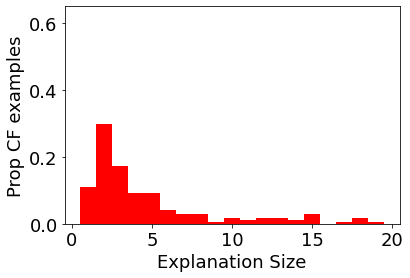
\includegraphics[scale=0.27]{04-research-cfgnn/images/tree-cycles-random.png}
    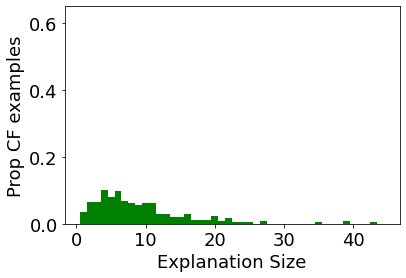
\includegraphics[scale=0.27]{04-research-cfgnn/images/tree-grid-random.png}
    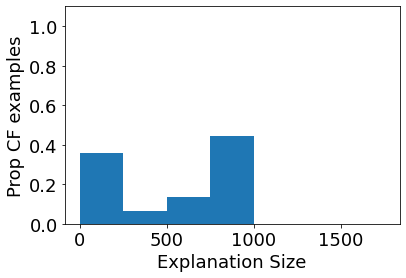
\includegraphics[scale=0.27]{04-research-cfgnn/images/ba-shapes-random.png}
    
        \caption{Histograms showing the proportion of counterfactual examples that have a certain explanation size from \baserand{}. Note the $x$-axis for \synone{} goes up to 1500. Left: \synfour{}, Middle: \synfive{}, Right: \synone{}.  }
        \label{fig:random-explanation-size}
        \bigskip \bigskip
        
    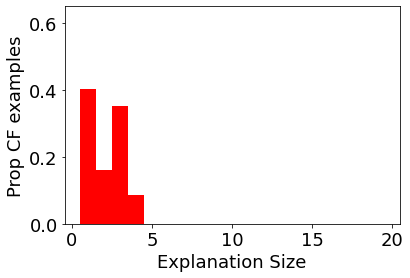
\includegraphics[scale=0.27]{04-research-cfgnn/images/tree-cycles-keep.png}
    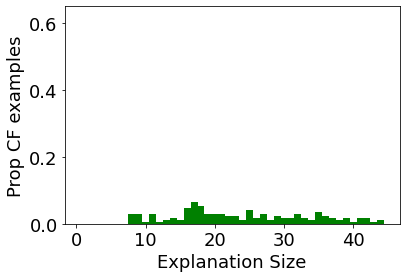
\includegraphics[scale=0.27]{04-research-cfgnn/images/tree-grid-keep.png}
    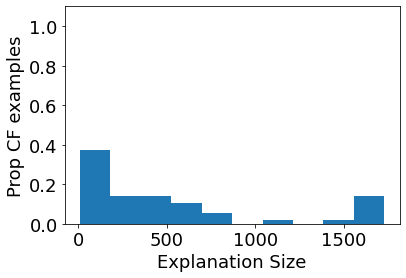
\includegraphics[scale=0.27]{04-research-cfgnn/images/ba-shapes-keep.png}
    
        \caption{Histograms showing the proportion of counterfactual examples that have a certain explanation size from \basekeep{}. Note the $x$-axis for \synone{} goes up to 1500. Left: \synfour{}, Middle: \synfive{}, Right: \synone{}. }
        \label{fig:keep-explanation-size}
        \bigskip \bigskip
        
        
    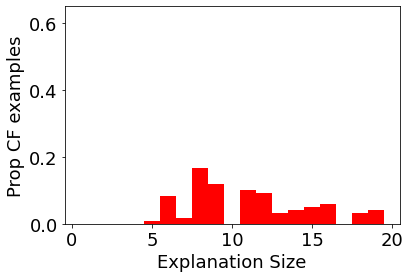
\includegraphics[scale=0.27]{04-research-cfgnn/images/tree-cycles-remove.png}
    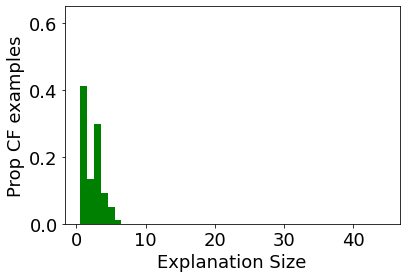
\includegraphics[scale=0.27]{04-research-cfgnn/images/tree-grid-remove.png}
    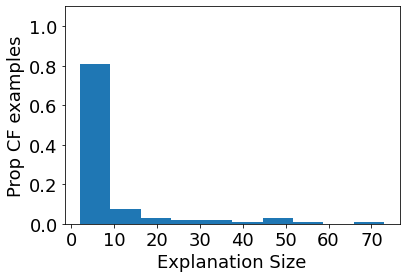
\includegraphics[scale=0.27]{04-research-cfgnn/images/ba-shapes-remove.png}
    
        \caption{Histograms showing the proportion of counterfactual examples that have a certain explanation size from \baserm{}. Note the $x$-axis for \synone{} goes up to 70. Left: \synfour{}, Middle: \synfive{}, Right: \synone{}. }
        \label{fig:remove-explanation-size}
        \bigskip \bigskip
        
    % 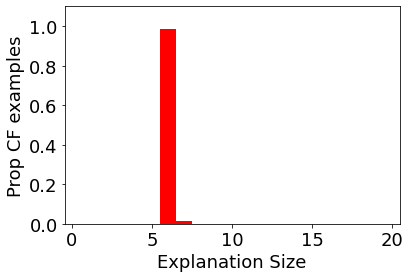
\includegraphics[scale=0.38]{images/tree-cycles-gnnexplainer.png}
    % 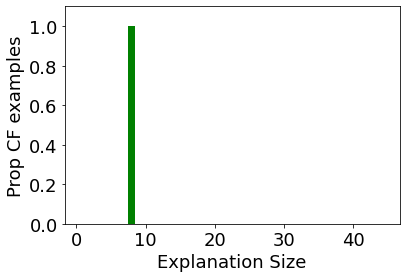
\includegraphics[scale=0.38]{images/tree-grid-gnnexplainer.png}
    % 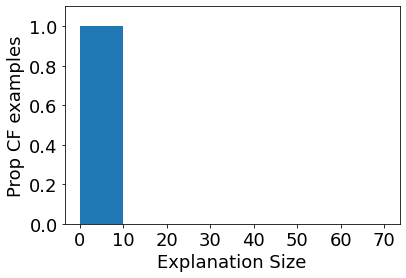
\includegraphics[scale=0.38]{images/ba-shapes-gnnexplainer.png}
    
    %     \caption{Histograms showing explanation size from \gnnexplainer{} for $S=$ GT. Note that the y-axis goes up to 1. Left: \synfour{}, Middle: \synfive{}, Right: \synone{}.}
    %     \label{fig:gnnexplainer-explanation-size}

    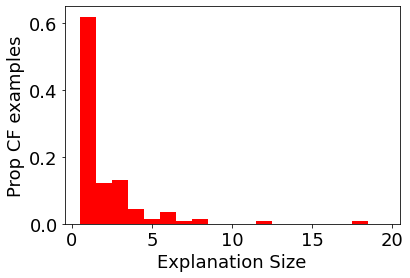
\includegraphics[scale=0.27]{04-research-cfgnn/images/tree-cycles.png}
    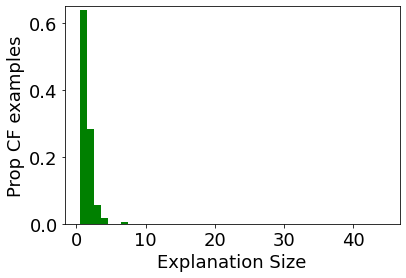
\includegraphics[scale=0.27]{04-research-cfgnn/images/tree-grid.png}
    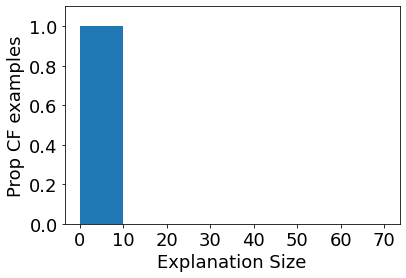
\includegraphics[scale=0.27]{04-research-cfgnn/images/ba-shapes.png}
    
        \caption{Histograms showing the proportion of counterfactual examples that have a certain explanation size from CF-GNNExplainer. Note the $x$-axis for \synone{} goes up to 70. Left: \synfour{}, Middle: \synfive{}, Right: \synone{}. }
        \label{fig:explanation-size}
        
\end{figure*}







\subsection{Comparison to \gnnexplainer{}}
Table~\ref{table:results-gnnexplainer} shows the results comparing our method to \gnnexplainer{}. We find that our method outperforms \gnnexplainer{} across all three datasets in terms of both fidelity and accuracy, for all tested values of $S$. 
However, this is not surprising since \gnnexplainer{} is not meant for generating counterfactual explanations, so we cannot expect it to perform well on a task it was not designed for. 
We cannot compare explanation size or sparsity fairly since \gnnexplainer{} requires the user to input the value of $S$. 



\begin{table*}[]
\centering
\caption{Results comparing our method to \gnnexplainer{}. \gnnexplainer{} cannot find $S$ automatically, so we try varying values of $S$. GT indicates the size of the ground truth explanation for each dataset. CF-GNNExplainer finds $S$ automatically. Below each metric, $\blacktriangledown$ indicates a low value is desirable, while $\blacktriangle$ indicates a high value is desirable.}
\label{table:results-gnnexplainer}
\setlength{\tabcolsep}{4pt}
\scriptsize{
\begin{tabular}{lrrrr rrrr rrrr}
\toprule
\multicolumn{1}{c}{} & \multicolumn{4}{c}{\synfour{}}                                                                                                                 & \multicolumn{4}{c}{\synfive{}}                                                                                                                   & \multicolumn{4}{c}{\synone{}}                                                                                                                  \\ 
\cmidrule(r){2-5}\cmidrule(r){6-9}\cmidrule{10-13} 
               & \multicolumn{1}{c}{Fid.} & \multicolumn{1}{c}{Size} & \multicolumn{1}{c}{Spars.} & \multicolumn{1}{c}{Acc.} & \multicolumn{1}{c}{Fid.} & \multicolumn{1}{c}{Size} & \multicolumn{1}{c}{Spars.} & \multicolumn{1}{c}{Acc.} & \multicolumn{1}{c}{Fid.} & \multicolumn{1}{c}{Size} & \multicolumn{1}{c}{Spars.} & \multicolumn{1}{c}{Acc.} \\
\gnnexpshort{} & \multicolumn{1}{c}{$\blacktriangledown$} &\multicolumn{1}{c}{$\blacktriangledown$} &\multicolumn{1}{c}{$\blacktriangle$} & \multicolumn{1}{c}{$\blacktriangle$} & \multicolumn{1}{c}{$\blacktriangledown$} &\multicolumn{1}{c}{$\blacktriangledown$} &\multicolumn{1}{c}{$\blacktriangle$} & \multicolumn{1}{c}{$\blacktriangle$} & \multicolumn{1}{c}{$\blacktriangledown$} &\multicolumn{1}{c}{$\blacktriangledown$} &\multicolumn{1}{c}{$\blacktriangle$} & \multicolumn{1}{c}{$\blacktriangle$} \\
\midrule


 $S=1$ & 0.65 & 1.00 & 0.92 & 0.61 & 0.69 & 1.00 & 0.96 & 0.79 & 0.90 & 1.00 & 0.94 & 0.52 \\
 $S=2$ & 0.59 & 2.00 & 0.85 & 0.54 & 0.51 & 2.00 & 0.92 & 0.78 & 0.85 & 2.00 & 0.91 & 0.40  \\
 $S=3$ & 0.56 & 3.00 & 0.79 & 0.51 & 0.46 & 3.00 & 0.88 & 0.79 & 0.83 & 3.00 & 0.87 & 0.34 \\
 $S=4$ & 0.58 & 4.00 & 0.72 & 0.48 & 0.42 & 4.00 & 0.84 & 0.79 & 0.83 & 4.00 & 0.83 & 0.31 \\
 $S=5$ & 0.57 & 5.00 & 0.66 & 0.46 & 0.40 & 5.00 & 0.80  & 0.79 & 0.81 & 5.00 & 0.81 & 0.27 \\
 $S=$ GT &  0.55 &	6.00 & 0.57 &	0.46 &	0.35 &	11.83 &	0.53 &	0.74 &	0.82 &	6.00 &	0.79 &	0.24    \\

\midrule
CF-GNN               & \textbf{0.21}                              & 2.09                     & 0.90                       & \textbf{0.94}                      & \textbf{0.07}                              & 1.47                     & 0.94                       & \textbf{0.96}                      & \textbf{0.39}                              & 2.39                     & 0.99                       & \textbf{0.96}                 \\
\bottomrule
\end{tabular}
}
\end{table*}


\subsection{Summary of Results} 
Evaluating on four distinct metrics for each dataset gives us a more holistic view of the results. 
We find that across all three datasets, CF-GNNExplainer can generate counterfactual examples for the majority of nodes in the test set (i.e., low fidelity), while only removing a small number of edges (i.e., low explanation size, high sparsity). For nodes where we know the ground truth (i.e., those in the motifs) we achieve at least 94\% accuracy. 

Although \baserand{} can generate counterfactual examples for every node, they are not very minimal or accurate. 
The latter is also true for \basekeep{} -- in general, it has the worst scores for explanation size, sparsity and accuracy. 
\gnnexplainer{} performs at a similar level as \basekeep{}, indicating that although it is a prominent GNN XAI method, it is not well-suited for solving the counterfactual explanation problem. 

\baserm{} is competitive in terms of explanation size, but it performs poorly in terms of fidelity for the \synfour{} and \synfive{} datasets, and its accuracy on these datasets is unknown since it is unable to generate \emph{any} counterfactual examples for nodes in the motifs. 
These results show that our method is simple and effective in solving the counterfactual explanation task, unlike the baselines we test. 










%%!TEX root = ../main.tex


\section{Conclusion}
\label{section:fact-conclusion}

In this chapter, we share our setup for the FACT-AI course at \OurUniversity{}, which teaches FACT-AI topics through reproducibility. 
The course set out to give students 
\begin{enumerate*}[label=(\roman*)]
    \item an understanding of FACT-AI topics, 
    \item an understanding of algorithmic harm, 
    \item familiarity with recent FACT-AI methods, and
    \item an opportunity to reproduce FACT-AI solutions, 
\end{enumerate*}
through a combination of lectures, paper discussion sessions and a reproducibility project. 
%
Through their projects, our students engaged with the open-source community by creating a public code repository (in the 2019--2020 iteration), as well as with the research community via successful submissions to the ML Reproducibility Challenge (in the 2020--2021 iteration). 
We also detail how the 2020--2021 iteration brought about its own unique set of challenges due to the COVID-19 pandemic. 

In this course, we illustrate that reproducibility should be viewed as a fundamental component of FACT-AI. 
We received very positive feedback on teaching FACT-AI topics through reproducibility. We believe this was an excellent fit for our students, which not only helped motivate them for the duration of the course, but also helped them develop skills that will be essential in their future research careers, whether in the private or public sector. 


With this final chapter, we answer \textbf{\ref{rq:pedagogy}}: we can use reproducibility as a mechanism for teaching responsible AI concepts to a technical, research-oriented audience. 
Structuring the course around a reproducibility project gives students the opportunity to learn about responsible AI concepts, such as explainability, in a hands-on manner. 
Since the publication of the paper on which this chapter is based \citep{lucic2022reproducibility}, we ran another iteration of the FACT-AI course in 2021--2022 under the same setup as the previous year, where students submitted their reports to the 2022 edition of the ML Reproducibility Challenge. 
21 of the 43 papers accepted to the ML Reproducibility Challenge in 2022 were from students in the FACT-AI course. 
These also included some awards: the Best Paper Award was awarded to a group from the FACT-AI course as well as 2 of the 4 Outstanding Paper Awards. 
We believe this indicates that our course setup can serve as a starting point for effective participation in the broader ML research community. 
%
\section{Results Table Including Standard Deviations}
Here we show Table 2 from the manuscript including standard deviations. 
We report standard deviation for two metrics: \textit{Explanation Size} and \textit{Sparsity}, since both of these involve taking the mean over the entire dataset. 
Standard deviation does not apply to \textit{Fidelity} or \textit{Accuracy} because these metrics represent a proportion as opposed to a mean. 


\begin{table}[h]
\centering
\caption*{Table 2: Results comparing our method (denoted \OurShort{}) to \baserand{}, \basekeep{}, and \baserm{}. Below each metric, $\blacktriangledown$ indicates a low value is desirable, while $\blacktriangle$ indicates a high value is desirable.}
\label{table:results}
%\setlength{\tabcolsep}{4pt}
%\footnotesize{
\resizebox{\textwidth}{!}{\begin{tabular}{lrrrrrrrrrrrr}
\toprule
\multicolumn{1}{c}{} & \multicolumn{4}{c}{\synfour{}}                                                                                                                 & \multicolumn{4}{c}{\synfive{}}                                                                                                                   & \multicolumn{4}{c}{\synone{}}                                                                                                                  \\ 
\cmidrule(r){2-5}\cmidrule(r){6-9}\cmidrule{10-13} 
               & \multicolumn{1}{c}{\textit{Fid.}} & \multicolumn{1}{c}{\textit{Size}} & \multicolumn{1}{c}{\textit{Spars.}} & \multicolumn{1}{c}{\textit{Acc.}} & \multicolumn{1}{c}{\textit{Fid.}} & \multicolumn{1}{c}{\textit{Size}} & \multicolumn{1}{c}{\textit{Spars.}} & \multicolumn{1}{c}{\textit{Acc.}} & \multicolumn{1}{c}{\textit{Fid.}} & \multicolumn{1}{c}{\textit{Size}} & \multicolumn{1}{c}{\textit{Spars.}} & \multicolumn{1}{c}{\textit{Acc.}} \\

% & \multicolumn{1}{c}{$\downarrow$} &\multicolumn{1}{c}{$\downarrow$} &\multicolumn{1}{c}{$\uparrow$} & \multicolumn{1}{c}{$\uparrow$} & \multicolumn{1}{c}{$\downarrow$} &\multicolumn{1}{c}{$\downarrow$} &\multicolumn{1}{c}{$\uparrow$} & \multicolumn{1}{c}{$\uparrow$} & \multicolumn{1}{c}{$\downarrow$} &\multicolumn{1}{c}{$\downarrow$} &\multicolumn{1}{c}{$\uparrow$} & \multicolumn{1}{c}{$\uparrow$} \\

Method & \multicolumn{1}{c}{$\blacktriangledown$} &\multicolumn{1}{c}{$\blacktriangledown$} &\multicolumn{1}{c}{$\blacktriangle$} & \multicolumn{1}{c}{$\blacktriangle$} & \multicolumn{1}{c}{$\blacktriangledown$} &\multicolumn{1}{c}{$\blacktriangledown$} &\multicolumn{1}{c}{$\blacktriangle$} & \multicolumn{1}{c}{$\blacktriangle$} & \multicolumn{1}{c}{$\blacktriangledown$} &\multicolumn{1}{c}{$\blacktriangledown$} &\multicolumn{1}{c}{$\blacktriangle$} & \multicolumn{1}{c}{$\blacktriangle$} \\
\midrule
\baserand{}               & \textbf{0.00}                     & 4.70   $\pm$       4.28                    & 0.79     $\pm$ 0.07                           & 0.63                               & \textbf{0.00}                     & 9.06    $\pm$ 6.81                          & 0.75      $\pm$ 0.07                          & 0.77                               & \textbf{0.00}                     & 503.31   $\pm$ 332.61                         & 0.58   $\pm$ 0.10                             & 0.17                              \\
\basekeep{}                 & 0.32                              & 15.64      $\pm$ 12.36                       & 0.13       $\pm$ 0.06                         & 0.45                               & 0.32                              & 29.30      $\pm$16.53                       & 0.09      $\pm$ 0.04                          & 0.72                               & 0.60                              & 504.18    $\pm$ 567.92                        & 0.05      $\pm$ 0.05                          & 0.18                              \\
\baserm{}              & 0.46                              & 2.11          $\pm$ 1.04                    & 0.89         $\pm$ 0.04                       & ---                                  & 0.61                              & 2.27         $\pm$ 1.28                     & 0.92      $\pm$ 0.04                          & ---                                  & 0.21                              & 10.56      $\pm$ 20.11                       & 0.97     $\pm$ 0.04                           & \textbf{0.99}                     \\


% \gnnexpshort{} ($S=$ GT) &  0.55 &	6.00 & 0.57 &	0.46 &	0.35 &	11.83 &	0.53 &	0.74 &	0.82 &	6.00 &	0.79 &	0.24    \\

\midrule
\OurShort{}               & 0.21                              & \textbf{2.09}     $\pm$ 2.21                & \textbf{0.90}    $\pm$ 0.07                   & \textbf{0.94}                      & 0.07                              & \textbf{1.47}    $\pm$0.77                 & \textbf{0.94}    $\pm$ 0.04                   & \textbf{0.96}                      & 0.39                              & \textbf{2.39}    $\pm$ 1.39                 & \textbf{0.99}      $\pm$ 0.01                 & 0.96                 \\
\bottomrule
\end{tabular}}
%}
\end{table}



All differences between \OurMethod{} and the baselines are statistically significant with $\alpha=0.01$ using a $t$-test, with two exceptions: \OurMethod{} vs. \baserm{} on the \synfive{} dataset, for (i) \textit{Explanation Size} and (ii) \textit{Sparsity}. However, \OurMethod{} outperforms \baserm{} significantly on \textit{Fidelity} and \textit{Accuracy} ($\alpha=0.01$). 


We do not calculate standard deviations for Table 3, where we compare against \gnnexplainer{}, since we cannot evaluate \gnnexplainer{} on \textit{Explanation Size} or \textit{Sparsity}. This is because the user must specify the \textit{Explanation Size} in advance (see Sections 6.2, 7.2). We can only evaluate \gnnexplainer{} on \textit{Fidelity} and \textit{Accuracy}, neither of which require standard deviation calculations since they represent proportions. 





\section*{Reproducibility}
To facilitate the reproducibility of the work in this chapter, our code is available at \url{https://github.com/gabriben/recfusion}.









%%% Local Variables:
%%% mode: latex
%%% TeX-master: "../thesis-main"
%%% End:
